\twocolumn[
\begin{center}
\title{\color[cmyk]{1, 0.57, 0, 0.38}{\Huge\bfseries Linea di comando\\}} % definisco il titolo dell'articolo
\author{\scriptsize Gabriele Trombini(mailga@fedoraonline.it)} % definisco l'autore e altre informazioni
\date{}
\end{center}
{\color[cmyk]{1, 0.46, 0, 0}\LARGE (Parte prima) Consolle virtuale e terminale - la base dei sistemi GNU/Linux}\\
\maketitle
\normalsize
\doublespacing
\hfill
]
\definecolor{shadecolor}{cmyk}{0, 0, 0, 0.8}
\onehalfspacing
\lettrine[lines=1, loversize=0.1, lraise=0.1]{\color[cmyk]{0.5, 0, 1, 0}\bfseries L}{}a linea di comando è sicuramente un ostacolo per chi si avvicina a Linux.\\

Se è vero che un utente smaliziato lavora, in molti casi, con la shell aperta, è altrettanto vero che molti nuovi utenti si trovano impreparati all'utilizzo di quello che è universalmente riconosciuto come uno strumento essenziale dei sistemi del pinguino.\\

Se vogliamo avvicinarci con la giusta sicurezza a questo strumento, dobbiamo tenere ben presente che:
\begin{itemize}
 \item {\itshape la shell è entusiasmante;}
 \item {\itshape la shell è potente;}
 \item {\itshape la shell non accetta la troppa confidenza.} 
\end{itemize}

Cominciamo con il fare chiarezza sui termini che normalmente vengono usati anche per definire la medesima cosa, ma che hanno significati differenti seppur minimi:

\begin{itemize}
 \item {\itshape terminale.}\\
Il terminale è lo strumento con il quale si comunica con il sistema (tastiera e monitor).
 \item {\itshape shell.}\\
La shell è l'interprete dei comandi immessi tramite terminale. In un sistema con
interfaccia grafica attiva (server X), la shell è ospitata all’interno
di un terminale emulato. 
 \item {\itshape consolle.} \\
La consolle è l'interfaccia testuale vera e propria, che si attiva al di fuori del server grafico. 
\end{itemize}

Nell'uso comune, per comodità, i tre termini vengono intesi come lo stesso strumento, ma in questo articolo faremo riferimento alla {\itshape shell}, presente in tutti di desktop environments ed in particolare alla {\itshape shell bash (bourne again shell)}, installata di default dal sistema e sicuramente la più utilizzata.\\

Esistono varie tipologie di shell, tutte con delle caratteristiche in comune, ma che hanno delle diferenze sostanziali apprezzate dai vari utenti più avanzati.\\

E' possibile verificare l'elenco delle shell installate con il comando:
\begin{shaded}
{\color[cmyk]{0, 0, 0, 0}\textdollar\ cat /etc/shells}
\end{shaded}

\begin{figure}[!htbp]
\centering
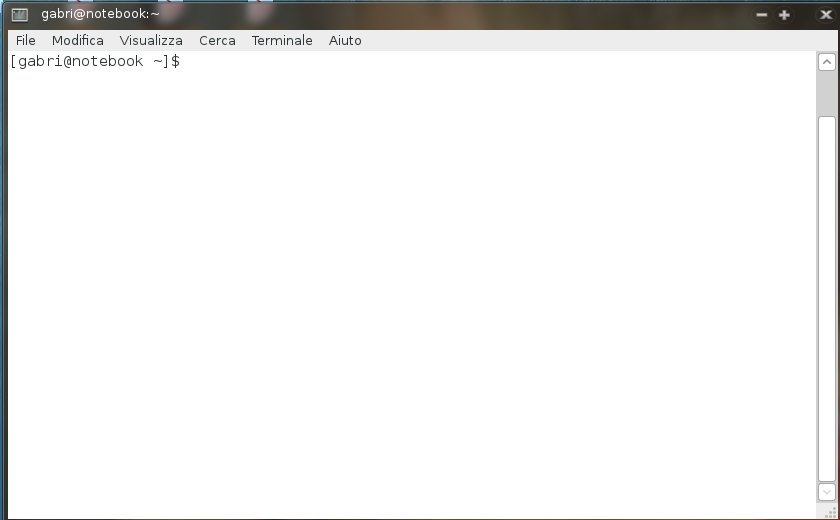
\includegraphics[scale=.30]{articoli/primi_passi/immagini/gnome_terminal.jpeg}
\caption{emulatore di terminale in Gnome (gnome terminal)\label{Fig.2: gnome_terminal}}
\end{figure}

\begin{center}
{\centering\bfseries La shell è entusiasmante}
\end{center}

Per chi arriva da altri sistemi operativi, dove l'interfaccia testuale è pressochè assente, si troverà spaesato di fronte alla necessità (talvolta assoluta) di dover aprire una shell per poter operare al meglio.\\

Dopo una normale diffidenza iniziale, in breve tempo avrà modo di apprezzare questo strumento basilare del sistema.\\

L'utente Linux è sempre spinto dalla curiosità e dalla voglia di capire ed è per questo che troverà molto piacevole appoggiarsi alla linea di comando.\\


\begin{figure*}[!htbp]
\centering
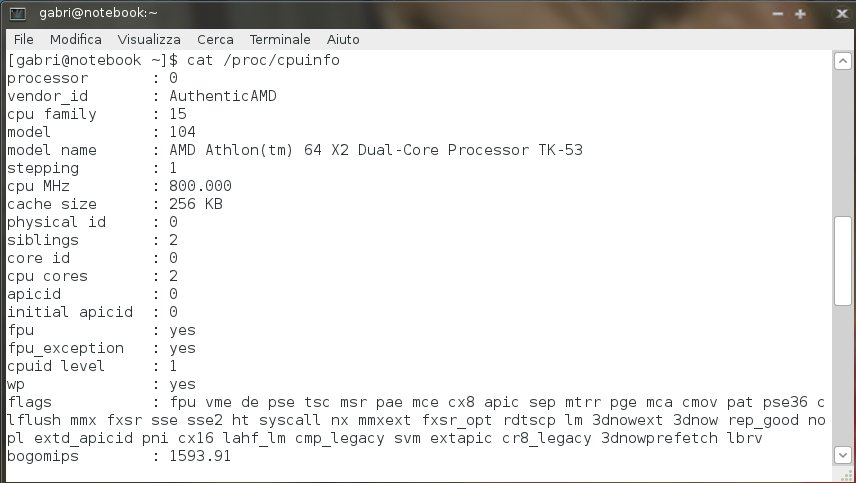
\includegraphics[scale=.60]{articoli/primi_passi/immagini/cpu_info.jpeg}
\caption{visualizzazione delle caratteristiche del processore in gnome-terminal\label{Fig.3: cpu_info}}
\end{figure*}


\begin{center}
{\bfseries La shell è potente}
\end{center}

A differenza delle interfacce grafiche, la shell permette una iterazione con il sistema molto elastica, arrivando in profondità fino ai processi vitali.\\

Tutto il sistema, con le dovute autorizzazioni, può essere modificato e analizzato per mezzo dei comandi e opzioni di programmi di utilità e software aggiuntivi.\\

Inoltre la shell è in grado di interpretare il proprio linguaggio di scripting ({\itshape bash scripting}) in cui la concatenazione di comandi e operatori può dare modo all'utente di automatizzare la propria attività.\\

\begin{center}
{\bfseries La shell non accetta la troppa confidenza}
\end{center}
Proprio per le qualità di cui sopra, corriamo il rischio di acquisire troppa confidenza con uno strumento che, a causa della sua caratteristica di iterazione anche a basso livello con il sistema, potrebbe indurci all'esecuzioni di operazioni senza la giusta dose di attenzione.\\

Si può arrivare a causare danni irreversibili alla propria station causando, spesso, perdite di dati, costringendoci ad un difficile recupero.\\

Non esiste un equilibrio oggettivo per questi fattori, il tutto è riconducibile alle proprie caratteristiche personali; di certo non bisogna temere il terminale ma sicuramente occorre avvicinarsi con piena coscienza di ciò che ci si accinge a fare.\\

Quindi il terminale ci consente di capire come funziona la nostra workstation ma, soprattutto, entriamo in sintonia con essa perchè ci permette di capire cosa stiamo facendo e cosa fa il sistema in risposta al nostro comando.\\

Chi ha acquisito una buona manualità sostiene che con il terminale si lavora molto velocemente; e non lo dicono solo i ``vecchi'' utilizzatori.\\

Aprendo la shell la riga che compare ({\itshape [gabri@notebook $\sim$]\textdollar}) è già fonte di alcune informazioni come il mio nome utente (gabri), il nome della mia macchina (notebook), in quale directory sono posizionato (la tilde $\sim$ indica che mi trovo all'interno della mia home, ovvero /home/gabri) ed infine il simbolo del dollaro (\textdollar), da distinguere da quello del cancelletto (\#) che sta a significare che ho acquisito le credenziali di root (quest'ultimo caso verrà trattato successivamente).\\

A questo punto il terminale è pronto ad accettare i comandi che vengono impartiti da tastiera.

\begin{figure*}[!t]
\centering
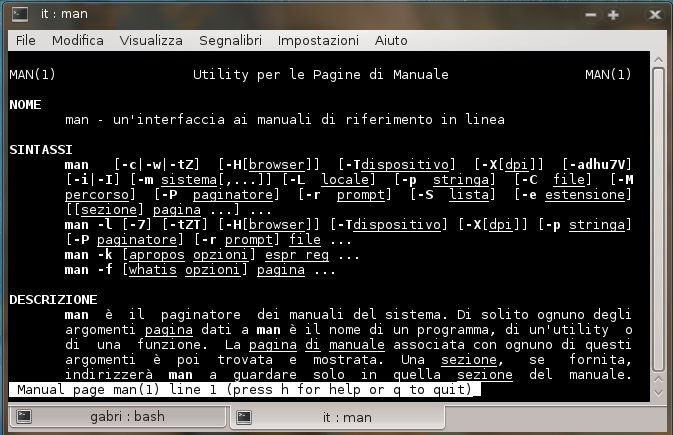
\includegraphics[scale=.80]{articoli/primi_passi/immagini/man_man.jpeg}
\caption{visualizzazione della pagina di manuale del comando {\itshape man}\label{Fig.4: man_man}}
\end{figure*}

\begin{shaded}
{\color[cmyk]{0, 0, 0, 0}\textdollar\ man nomecomando}
\end{shaded}
Utilizzando il comando qui sopra, appare all'interno del terminale virtuale il manuale di istruzione per l'utilizzo del comando dato come argomento; è sempre bene studiarlo per destreggiarsi nell'esecuzione secondo le nostre aspettative.\\

Già l'abituarsi alla lettura delle pagine {\itshape man} è un ottimo inizio, ma sicuramente il poter finemente configurare l'applicazione del comando mediante le opzioni rende molto interessante l'utilizzo della linea di comando.\\

Ovviamente il consiglio è quello di cimentarsi in esperimenti con comandi che non possono causare danni al sistema (come il comando {\itshape ls} oppure {\itshape cat} oppure lo stesso {\itshape man}), sebbene, utilizzando come utente e non come superuser, tali danni sarebbero circoscritti alla sola {\itshape /home} dell'utente stesso.\\

La {\itshape Bash} è inoltre fornita di completamento automatico; ci basta scrivere le lettere di inizio del comando per avere, premendo due volte il tasto {\itshape tab}, l'elenco completo dei comandi che iniziano con quelle lettere che ho premuto.\\
E' possibile, inoltre, usare la {\itshape history} per ripercorrere ed eventualmente selezionare gli ultimi comandi dati mediante l'utilizzo dei tasti ``freccia su'' e ``freccia giù''.\\

Da linea di comando è possibile anche avviare i programmi, anche quelli grafici, semplicemente inserendo il nome dell'eseguibile prima dell'invio:

\begin{shaded}
{\color[cmyk]{0, 0, 0, 0}\textdollar\ eseguibile}
\end{shaded}

come in questo caso specifico in cui lanciamo il web browser {\itshape firefox}, senza opzioni:

\begin{shaded}
{\color[cmyk]{0, 0, 0, 0}\textdollar\ firefox}
\end{shaded}

L'avvio dell'applicazione da terminale è utile soprattutto per un primo debug nel caso di malfunzionamento del lanciatore grafico, che invece non darebbe alcuna informazione aggiuntiva (l'applicazione non partirebbe e basta), mentre l'errore che viene segnalato in output è fondamentale per poter circostanziare il problema.\\

Autenticandoci come utenti, abbiamo delle restrizioni per quanto concerne la modifica o anche solo la visualizzazione dei file di sistema, proprio per evitare che, accidentalmente o meno, possa venire compromessa l'operatività della nostra stazione di lavoro.\\

Per interagire appieno occorre pertanto avere le credenziali del {\itshape superuser} (utente {\itshape root} che invece gode dei più ampi permessi.\\

Per diventare utente root occorre digitare al prompt:
\begin{shaded}
{\color[cmyk]{0, 0, 0, 0}\textdollar\ su}
\end{shaded}
e ci verrà richiesta la password assegnata all'utente root che, una volta inserita, ci permette di avere quei permessi necessari per l'amministrazione del sistema.

Da notare che, per motivi di sicurezza, alla digitazione della password di autenticazione, non si vedrà il cursore e che il prompt, come detto in precedenza, riporta il simbolo del cancelletto (\#).

\begin{figure}[!ht]
\centering
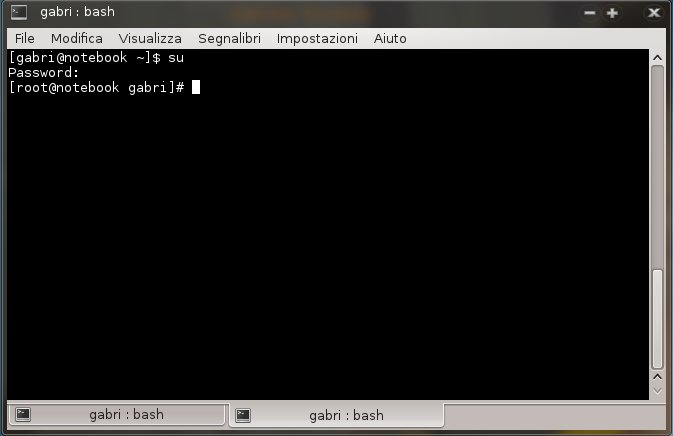
\includegraphics[scale=.35]{articoli/primi_passi/immagini/root.jpeg}
\caption{autenticazione di root}
\end{figure}

Eccoci autenticati come root nell'ambiente dell'utente (l'autenticazione con l'importazione dell'ambiente di root sarà oggetto di prossimi approfondimenti).\\

\hfill {\itshape (fine prima parte)}